\documentclass[10pt]{beamer}

% Preámbulo
\mode<presentation>{\usetheme{Frankfurt}}

%\setbeamertemplate{footline}[frame number]
%\useoutertheme[footline=institutetitle]{miniframes}

\setbeamertemplate{footline}
{%
\begin{beamercolorbox}[frame number]{section in head/foot}
\vskip2pt\insertshortauthor[width=0.3\linewidth,center,respectlinebreaks]\insertshorttitle[width=0.8\linewidth,center,respectlinebreaks]\insertframenumber/\inserttotalframenumber\vskip2pt
\end{beamercolorbox}%
}

% Justificar texto (hay que poner \justifying dentro de cada entorno, por ejemplo: itemize, enumerate,...)
%\usepackage{ragged2e}
%\justifying



% Incluye el fichero con la configuración de estilo (paquetes, idiomas, ...)
% PAQUETES

% Formato de los márgenes
%\usepackage{anysize}								% Obsoleto.
%\marginsize{2.5cm}{2.5cm}{2.5cm}{2.5cm}
%\usepackage[margin=2.5cm, nohead]{geometry}

% Tipografía
%\usepackage{mathptmx}					% Tipo de letra 'Times'.

% Codificación
\usepackage[utf8x]{inputenc}			% Permite el uso de caracteres acentuados.
\usepackage[T1]{fontenc}				% Letras acentuadas reales y no imitadas.
\usepackage{textcomp}					% Incluye mayor número de letras con diacríticos.

% Idiomas
\usepackage[english, spanish]{babel} 	% Para generar documentos en idiomas distintos al inglés.
%\usepackage{eurosym}					% Símbolo del euro (€).

% Espaciado
%\usepackage[onehalfspacing]{setspace}	% Controla el espaciado entre líneas.
										% \singlespacing, \onehalfspacing, \doublespacing
% Gráficos e imágenes
\usepackage{graphicx}
%\usepackage{subfig}					% Subfiguras: (a), (b),...

% Directorios con las imágenes
%\graphicspath{{contenido/cap3/imagenes}}

% Extensiones de las imágenes
%\DeclareGraphicsExtensions{eps}

% Otros paquetes
%\usepackage{latexsym} 					% Símbolos extra.
%\usepackage{dsfont}						% Otros símbolos: \mathds{I}
%\usepackage{marvosym}					% Otros símbolos: \Gemini

% La mayoría de los símbolos matemáticos se incluyen gracias al paquete amsmath. Además, con los paquetes latexsymb y amssymb se completa la lista de todos los símbolos, operadores y delimitadores posibles. 
%\usepackage{amsmath}
%\usepackage{amssymb}

% Enlaces en el pdf. (Cuidado con usar imagenes .eps y este paquete, consultar documentación).
%\usepackage[dvipdfm]{hyperref}


% Reutilizar contadores de enumerate.
%\usepackage{enumerate}
%\usepackage{enumitem}

% Apéndices
%\usepackage{appendix}

% Bibliografía en español
%\usepackage[spanish]{flexbib}
%\usepackage[fixlanguage]{babelbib}	%[spanish,fixlanguage]
%\usepackage{custom-bib}
%\selectbiblanguage{spanish}

% Para poner varias bibliografías y/o referencias
%\usepackage{multibib}
%\newcites{ref}{Referencias}

% PARTICIÓN DE SÍLABAS
%\hyphenation{sis-te-má-ti-co pa-leo-lí-ti-co}
%\hyphenation{VALOR MINIMAX}

% Redefinición de nombres
%\renewcommand{\appendixname}{Apéndices}
%\renewcommand{\appendixtocname}{Apéndices}
%\renewcommand{\appendixpagename}{Apéndices}
%\renewcommand{\tablename}{Tabla}

% Para que aparezca las subsubsecciones numeradas:
%\setcounter{secnumdepth}{3}
%\setcounter{tocdepth}{3}

%\usefonttheme{default}

% Información
\title[Entorno interactivo para el estudio de estrategias de I.A. en juegos]{Entorno interactivo para el estudio de estrategias de I.A. en juegos}
\author{José Miguel Horcas Aguilera}
\date{\today}


%\includeonly{}
%\makeindex

\AtBeginSection[]
{
\begin{frame}<beamer>
\frametitle{Índice}
\tableofcontents[currentsection,currentsubsection]
\end{frame}
}

% Colores
\definecolor{verde}{rgb}{0.1,0.6,0.1}
\definecolor{rojo}{rgb}{0.6,0.1,0.1}

\begin{document}	% inicio 

% Título
\begin{frame}[plain]
	\titlepage
\end{frame}
%\frame{\titlepage}

% Índice
\section*{Índice}
\begin{frame}
 \frametitle{Índice}
  \tableofcontents%[part=1,pausesections]
\end{frame}

%%------------------------------------------------------------------------------
% INTRODUCCIÓN
\section{Introducción}
\label{sec:introduccion}

%\frame {\tableofcontents[sec:introduccion]}

% Transparencia Introducción
\begin{frame}[t]
\frametitle{Introducción}
%\framesubtitle{SubIntroducción}
\begin{block}{Objetivos}
Desarrollar un entorno interactivo que permita jugar, estudiar y comparar el rendimiento de estrategias de IA en juegos.
\end{block}

\begin{block}{Motivación}
%Los juegos son un tema atractivo en IA:
\begin{itemize}
	\item Facilidad de representar el estado de los juegos.
	\item Definición precisa de las reglas.
%	\item Demasiado difíciles para resolverlos.
	\item Requieren la capacidad de tomar alguna decisión.
%	\item Los algoritmos pueden extenderse a otras áreas.
\end{itemize}
\end{block}

\end{frame}

%%------------------------------------------------------------------------------
% JUEGOS
\section{Juegos}

% Transparencia juegos (I)
\begin{frame}[t]
\frametitle{Juegos}
\begin{block}{Características de los juegos}
Bipersonales, por turnos, de suma cero, de información perfecta y deterministas.
%%los juegos a considerar son aquellos que presenten entornos deterministas,
%%totalmente observables en los cuales hay dos agentes cuyas acciones deben alternar %y en los que los valores de utilidad al final son iguales y opuestos.
\end{block}

\begin{exampleblock}{Ejemplos: \textit{classic board-games}}
	\begin{columns}

		\begin{column}{0.5\linewidth}
\begin{itemize}
\item 3 en raya
\item \textbf{Conecta-4}
\item Damas
\item Othello (Reversi)
\item Ajedrez
\item \textbf{Go}
\end{itemize}
		\end{column}
		\begin{column}{0.5\linewidth}
			\begin{figure}[t]
				\centering
				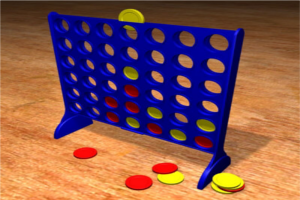
\includegraphics[scale=0.4]{imagenes/connect4.png}
				\label{fig:conecta4}
			\end{figure}
			\begin{figure}[t]
				\centering
				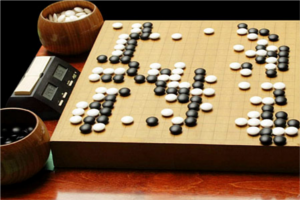
\includegraphics[scale=0.2]{imagenes/go.png}
				\label{fig:go}
			\end{figure}			
		\end{column}

	\end{columns}
\end{exampleblock}

\end{frame}
%%------------------------------------------------------------------------------
% Transparencia juegos (Conecta-K)
\begin{frame}[t]
\frametitle{Conecta-4}
%\framesubtitle{Conecta-4}
\begin{block}{Reglas}
{\small
\begin{itemize}
\item \textbf{Objetivo:}
Colocar 4 fichas en línea del mismo color. %(horizontal, vertical o diagonal). 
\item \textbf{Tablero:} 6x7.
\item Las fichas se dejan caer por las columnas.
\end{itemize}
%Versión generalizada: \textit{n} filas $\times$ \textit{m} columnas, \textit{K} fichas conectadas.
}
\end{block}

\begin{figure}[t]
\centering
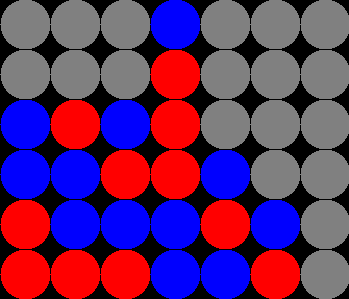
\includegraphics[scale=0.4]{imagenes/conecta4.png}
\label{fig:conecta4_aplicacion}
\end{figure}
			
\end{frame}

%%------------------------------------------------------------------------------
% Transparencia juegos (Go)
\begin{frame}[squeeze]
\frametitle{Go}
\begin{block}{Reglas}

\begin{itemize}
\item \textbf{Objetivo:}
controlar más tablero que el oponente.%una porción más grande del tablero que el oponente.
\item \textbf{Tablero:} 19$\times$19, 17$\times$17, 13$\times$13, \textbf{9$\times$9}.
\item Las fichas se colocan sobre las intersecciones.
\item Se capturan las fichas encerradas.
\item Prohibido repetir situaciones y suicidarse.
\item Gana el jugador con más puntos:
\begin{itemize}
	\item \textbf{Reglas japonesas:} $1p/inter. - 1p/fichacapturada$
	\item \textbf{Reglas chinas:} $1p/inter. + 1p/fichatablero$
\end{itemize}
\end{itemize}

\end{block}
\begin{figure}[t]
\centering
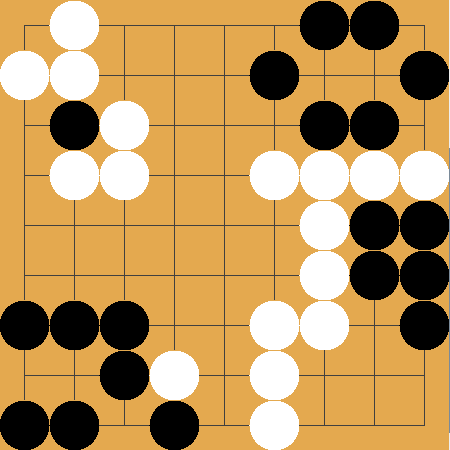
\includegraphics[scale=0.25]{imagenes/juego_go.png}
\label{fig:go_aplicacion}
\end{figure}

\end{frame}


%%------------------------------------------------------------------------------
% Transparencia juegos (II)
\begin{frame}[squeeze]
\frametitle{Problemas de búsqueda con adversarios}

%Los juegos se representan como problemas de búsqueda entre adversarios con los siguientes elementos:
\begin{block}{Representación de los juegos}
\begin{itemize}
\item \textbf{Estado inicial}: situación inicial de la partida y turno del jugador.
\item \textbf{Función sucesor}: movimiento legal y el estado resultante.
\item \textbf{Test terminal}: ¿cuándo se termina el juego?
\item \textbf{Función de utilidad}: +1, -1 ó 0 si el resultado es un triunfo, una pérdida o un empate.
\end{itemize}
\end{block}

\begin{figure}[h]
	\centering
	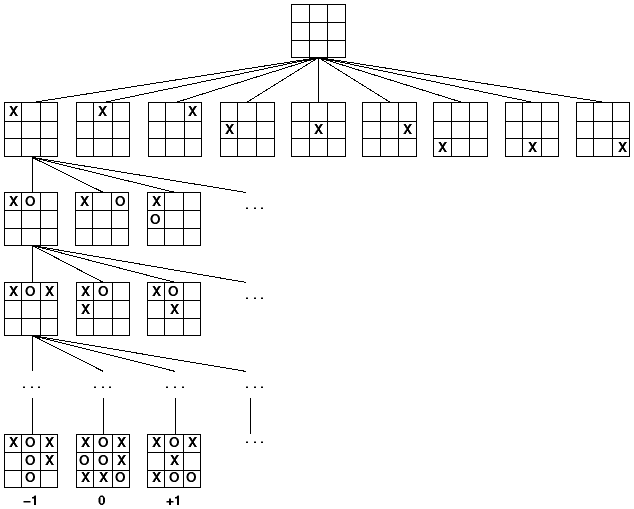
\includegraphics[scale=0.25]{imagenes/game_tree.png}
	%\caption{Árbol parcial de búsqueda para el \textit{3 en Raya}.}
	\label{fig:arbol_juego_3enraya}
\end{figure}

\end{frame}

%%------------------------------------------------------------------------------
% ESTRATEGIAS
\section{Estrategias y heurísticos}

% Transparencia Estrategias
%\begin{frame}[t]
%\frametitle{Agentes inteligentes}
%\begin{block}{}
%Un \textbf{agente inteligente} es un sistema capaz de percibir su entorno, procesar tales percepciones y actuar de manera racional.
%\end{block}
%\begin{block}{Agentes para juegos}
%\begin{itemize}
%\item \textbf{Medio}: espacio de estados de un juego.
%\item \textbf{Objetivo}: ganar el juego.
%\item \textbf{Percepciones}: percibe el estado del juego antes de realizar cada movimiento.
%\item \textbf{Acciones}: movimientos válidos del juego.
%\item \textbf{Conocimiento}: \textit{estrategia} para proponer un movimiento según las reglas del juego.
%\end{itemize}
%\end{block}
%
%\end{frame}
%%------------------------------------------------------------------------------
\begin{frame}[squeeze]
\frametitle{Estrategias}
%\begin{block}{Agentes para juegos}
%
%\begin{itemize}
%\item \textbf{Medio}: espacio de estados de un juego.
%\item \textbf{Objetivo}: ganar el juego.
%%\item \textbf{Percepciones}: percibe el estado del juego antes de realizar cada movimiento.
%\item \textbf{Acciones}: movimientos válidos del juego.
%\item \textbf{Conocimiento}: \textit{estrategia} para proponer un movimiento.
%\end{itemize}
%
%\end{block}

\begin{exampleblock}{Estrategias desarrolladas}
{\footnotesize
\begin{columns}
\begin{column}{0.4\linewidth}
\begin{itemize}
\item Humana
\item Aleatoria
\item Monte-Carlo
\item Monte-Carlo Tree Search
\end{itemize}
\end{column}
\begin{column}{0.4\linewidth}
\begin{itemize}
\item Evaluador heurístico
\item Minimax
\item Poda Alfa-Beta
\item Tablas de transposición
\end{itemize}
\end{column}
\end{columns}
}
\end{exampleblock}

%\begin{block}{Versiones}
{\footnotesize
\begin{center}
\begin{tabular}{lp{1cm}p{1cm}p{1cm}p{1cm}}
\hline
 & \multicolumn{4}{c}{\textbf{Parámetros}}\\
\textbf{Jugadores} & Prof. búsqueda & Nº simulaciones & Límite tiempo & Heurísticos\\
\hline
Aleatorio &  & & & \\
Monte-Carlo & & X & X & \\
Monte-Carlo Tree Search & & X & X  & \\
Evaluador heurístico & & & & X \\ 
Minimax & X & & X & X \\
Alfa-Beta & X & & X & X \\ 
Minimax (tabla transposición) & X & & X & X \\ 
Alfa-Beta (tabla transposición) & X & & X & X \\
\hline
\end{tabular}
\end{center}
}
%\end{block}
\end{frame}

%%------------------------------------------------------------------------------
\begin{frame}[t]
\frametitle{Estrategias básicas}

% Jugador humano
{\huge Jugador Humano}
\begin{block}{Estrategia}
Pide el movimiento a realizar por un dispositivo de entrada/salida.
\\
\textcolor{rojo}{Depende del juego.}
\end{block}

\bigskip

\bigskip

% Jugador aleatorio
{\huge Jugador aleatorio}
\begin{block}{Estrategia}
Realiza movimientos aleatorios.
\\
\textcolor{verde}{Es totalmente independiente del juego.}
\end{block}

\end{frame}

%%------------------------------------------------------------------------------
\begin{frame}[squeeze]
\frametitle{Agentes basados en simulaciones}

% Jugador monte-carlo
{\huge Monte-Carlo}
%\begin{block}{}
%Realiza simulaciones a partir del estado actual.
%\\
%Una \textbf{simulación} es una partida completa con movimientos al azar.
%\end{block}

\begin{block}{Estrategia}
{\small
%\begin{columns}
%		\begin{column}{0.5\linewidth}
%		\begin{itemize}
%			%\item Para cada posible movimiento realiza miles de simulaciones, obteniendo el valor de recompensa.		
%			\item Realiza simulaciones a partir del estado actual.
%			\item Una \textbf{simulación} es una partida completa con movimientos al azar.
%			\item El movimiento con mayor valor de recompensa esperado es el elegido.
%		\end{itemize}
%		\end{column}
%		\begin{column}{0.3\linewidth}
%\begin{figure}[t]
%\centering
%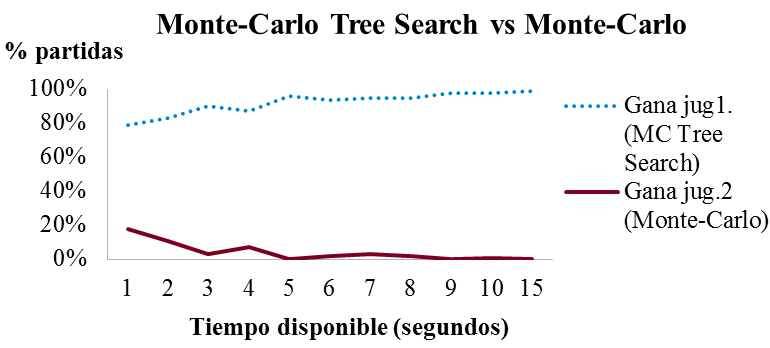
\includegraphics[scale=0.4]{imagenes/montecarlo2.png}
%\label{fig:jug_montecarlo}
%\end{figure}
%
%		\end{column}
%\end{columns}
\begin{itemize}
			%\item Para cada posible movimiento realiza miles de simulaciones, obteniendo el valor de recompensa.		
			\item Realiza simulaciones a partir del estado actual.
			\item Una \textbf{simulación} es una partida completa con movimientos al azar.
			\item El movimiento con mayor valor de recompensa esperado es el elegido.
		\end{itemize}
\begin{figure}[t]
\centering
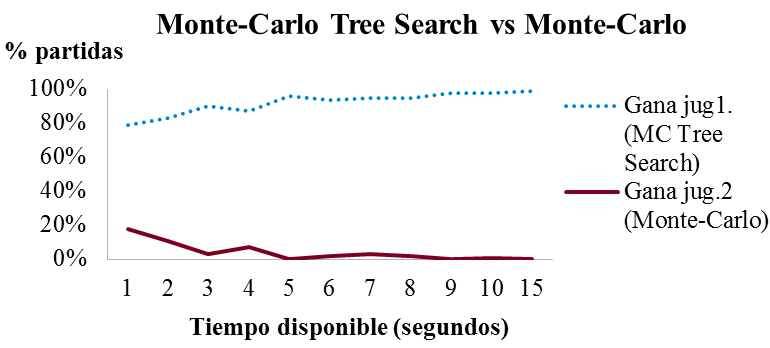
\includegraphics[scale=0.4]{imagenes/montecarlo2.png}
\label{fig:jug_montecarlo}
\end{figure}		
}
\end{block}

{\footnotesize 
\begin{exampleblock}{Versiones}
\begin{itemize}
	\item Número de simulaciones.
	\item Tiempo limitado.
\end{itemize}
\end{exampleblock}
}
\end{frame}

%%------------------------------------------------------------------------------
\begin{frame}[squeeze]
\frametitle{Agentes basados en simulaciones}

% Jugador monte-carlo
%\begin{block}{}
%Realiza simulaciones para decidir el mejor movimiento.
%\\
%Crea un \textbf{árbol de búsqueda} con la información de las simulaciones.
%\end{block}
{\huge Monte-Carlo Tree Search}
\begin{block}{Estrategia}
{\small
\begin{figure}[t]
\centering
\includegraphics[scale=0.35]{imagenes/montecarloTS.png}
\label{fig:jug_montecarloTS}
\end{figure}
}
\end{block}

{\footnotesize 
\begin{columns}
\begin{column}{0.5\linewidth}
\begin{exampleblock}{Parámetros}
\begin{itemize}
	\item Constante de exploración.
	\item Posibilidad de reutilizar el árbol.
\end{itemize}
\end{exampleblock}
\end{column}
\begin{column}{0.5\linewidth}
\begin{exampleblock}{Versiones}
\begin{itemize}
	\item Número de simulaciones.
	\item Tiempo limitado.
\end{itemize}
\end{exampleblock}
\end{column}
\end{columns}
}
\end{frame}

%%------------------------------------------------------------------------------
\begin{frame}[t]
\frametitle{Agentes con evaluador heurístico}

% Jugador evaluador
%\begin{block}{}
%Evalúan heurísticamente si una situación dada es favorable o no.
%\end{block}
%
%\begin{alertblock}{}
%Necesita de una función de evaluación heurística.
%\end{alertblock}

{\huge Evaluador heurístico}
\begin{block}{Estrategia}
\textit{Dado un estado, considera todos los movimientos inmediatos, los evalúa heurísticamente y escoge el mejor.}
\begin{figure}[t]
\centering
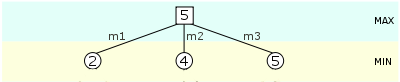
\includegraphics[scale=0.5]{imagenes/evaluadorHeuristico.png}
\label{fig:jug_evaluador}
\end{figure}
\end{block}

%Cualquier jugador que necesite de un heurístico puede considerarse
%como una especialización de este agente.

\end{frame}

%%------------------------------------------------------------------------------
\begin{frame}[squeeze]
\frametitle{Agentes con evaluador heurístico}

% Jugador minimax
%\begin{block}{}
%Proporciona una estrategia óptima (impracticable).
%% aunque en la práctica no es factible calcularla para juegos complejos.
%%Una estrategia óptima conduce a resultados al menos tan buenos como cualquier otra estrategia cuando uno juega con un oponente infalible.
%\end{block}
{\huge Minimax}
\begin{block}{Estrategia}
%Dado un estado:
%\begin{enumerate}
%	\item Genera el árbol de juegos completo a una determinada profundidad.
%	\item Evalúa heurísticamente los estados de ese nivel.
%	\item Los valores se propagan hacia arriba:
%	\begin{itemize}
%		\item Un nodo MAX toma como valor el máximo de sus hijos.
%		\item Un nodo MIN toma como valor el mínimo de sus hijos.
%	\end{itemize}
%	\item Se escoge el movimiento inmediato mejor valorado.
%\end{enumerate}
\begin{figure}[t]
\centering
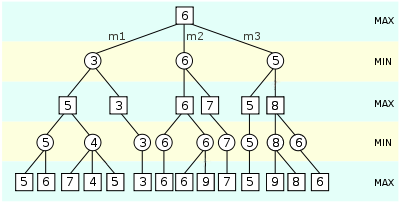
\includegraphics[scale=0.5]{imagenes/minimax.png}
\label{fig:jug_minimax}
\end{figure}
%Variante equivalente: \textbf{negamax}.
\end{block}

{\footnotesize 
\begin{exampleblock}{Versiones}
\begin{itemize}
	\item Profundidad máxima de búsqueda.
	\item Tiempo limitado.
\end{itemize}
\end{exampleblock}
}

\end{frame}

%%------------------------------------------------------------------------------
\begin{frame}[squeeze]
\frametitle{Agentes con evaluador heurístico}

% Jugador alfa-beta
%\begin{block}{}
%Calcula el mismo movimiento que minimax sin mirar los nodos que no influyen en la decisión final.
%\end{block}
{\huge Poda alfa-beta}
\begin{block}{Estrategia}
\begin{figure}[t]
\centering
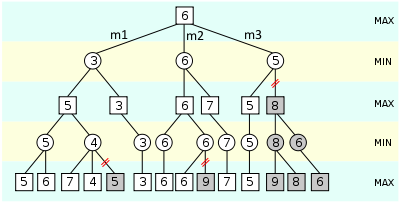
\includegraphics[scale=0.5]{imagenes/podaalfabeta.png}
\label{fig:jug_podaAlfaBeta}
\end{figure}
\end{block}

{\footnotesize 
\begin{exampleblock}{Versiones}
\begin{itemize}
	\item Profundidad máxima de búsqueda. % busqueda en profundidad (backtracking).
	\item Tiempo limitado.	% profundización progresiva.
\end{itemize}
\end{exampleblock}
}

\end{frame}

%%------------------------------------------------------------------------------
\begin{frame}[squeeze]
\frametitle{Agentes con evaluador heurístico}

% Jugador con tabla de transposición
%\begin{block}{}
%Una \textbf{transposición} es una permutación diferente de una secuencia de movimientos que termina en la misma posición.
%\\
%Una \textbf{tabla de transposición} almacena los resultados de búsquedas previas.
%\end{block}

{\huge Tabla de transposición}
\begin{block}{Estrategia}
{\footnotesize 
Una \textbf{transposición} es un estado que puede ser alcanzado por más de un camino.
}
\begin{figure}[t]
\centering
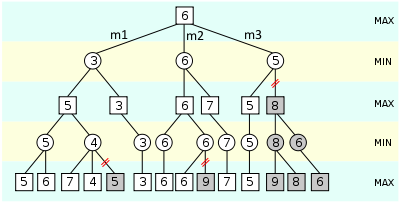
\includegraphics[scale=0.5]{imagenes/podaalfabeta.png}
\label{fig:jug_tablaTransposicion}
\end{figure}
\end{block}

%\begin{block}{Estrategia}
%\begin{itemize}
%\item Tabla hash con los estados previamente evaluados.
%\item Cuando aparece una transposición, se consulta en la tabla qué se determinó la última vez.
%\item Evita repetir de nuevo toda la búsqueda.
%\end{itemize}
%\end{block}

{\footnotesize 
\begin{exampleblock}{Versiones}
\begin{itemize}
	\item Minimax con tabla de transposición.
	\item Poda alfa-beta con tabla de transposición.
\end{itemize}
\end{exampleblock}
}

\end{frame}


%%------------------------------------------------------------------------------
% HEURÍSTICOS
%\section{Heurísticos}

% Transparencia Heurísticos
\begin{frame}[squeeze]
\frametitle{Heurísticos}
\begin{block}{Función de evaluación heurística}
\begin{displaymath}
e(n) = \left\{\begin{array}{ll}
\infty & \textnormal{si \textit{n} es un estado terminal y gana \textit{MAX}}\\
>0 & \textnormal{si \textit{n} es favorable para \textit{MAX}}\\
0 & \textnormal{si \textit{n} es indiferente (``empate'')}\\
<0 & \textnormal{si \textit{n} es desfavorable para \textit{MAX}}\\
-\infty & \textnormal{si \textit{n} es un estado terminal y pierde \textit{MAX}}\\
\end{array}\right.
\end{displaymath}
\end{block}

\begin{exampleblock}{Evaluadores heurísticos}
\begin{itemize}
\item Tabla de valor
\item Red neuronal
\item Heurísticos del Conecta-4:
\begin{itemize}
	\item Matriz de posibilidades
\end{itemize}
\item Heurísticos del Go:
\begin{itemize}
	\item Evaluador de territorios
	\item Evaluador de puntos JP
	\item Evaluador de puntos CH
\end{itemize}
\end{itemize}
\end{exampleblock}

\end{frame}

%%------------------------------------------------------------------------------
% Transparencia aprendizaje
%\begin{frame}[t]
%\frametitle{Aprendizaje}
%\begin{block}{Aprendizaje con refuerzo}
%\begin{itemize}
%	\item El agente aprende a base de ensayo-error.
%	\item El agente no necesita conocimiento del entorno.
%	\item El agente necesita una recompensa.
%	\item Método de las \textbf{Diferencias Temporales}:
%\begin{displaymath}
%U(n) = U(n) + \alpha(R(n) + U(s) - U(n))
%\end{displaymath}
%\end{itemize}
%\end{block}
%
%\begin{exampleblock}{Parámetros de entrenamiento}
%\begin{itemize}
%	\item Número de partidas.
%	\item Número de partidas entre cada pausa.
%	\item Número de pruebas en cada pausa.
%	\item Probabilidad de exploración.	
%	%Para garantizar que se obtiene una buena estrategia, se pueden realizar movimientos exploratorios durante el entrenamiento. Para ello se introduce una componente aleatoria para los movimientos del evaluador a entrenar: cada movimiento tendrá una probabilidad de ser aleatorio (exploratorio); en caso de que el movimiento sea exploratorio, no se entrenará al evaluador.
%\end{itemize}
%\end{exampleblock}
%
%\end{frame}

%%------------------------------------------------------------------------------
% Transparencia tabla de valor
\begin{frame}[squeeze]
\frametitle{Heurísticos genéricos}
\begin{block}{Tabla de valor}
{\small
\begin{itemize}
	\item $e(n) = tabla(n)$
	%\item Tabla con los valores de utilidad de cada estado.
	%Implementa la función de evaluación mediante una tabla con los valores de utilidad.
	\item Aprendizaje mediante el método de las diferencias temporales:
	\begin{displaymath}
tabla(n) \leftarrow tabla(n) + \alpha(tabla(s) - tabla(n))
\end{displaymath}
	%\item Los valores de la tabla se actualizan en cada paso del entrenamiento.
	\item \textcolor{verde}{Evaluador independiente del juego.}
\end{itemize}
}
\end{block}

\begin{block}{Red neuronal}
{\small
\begin{columns}
\begin{column}{0.4\linewidth}
\begin{itemize}
\item $e(n) = p_1 - p_2$
%\item Aprendizaje mediante retropropagación.
\item Método de las diferencias temporales.
\item \textcolor{rojo}{Depende del juego.}
\end{itemize}
%Red neuronal multicapa con aprendizaje mediante retropropagación.
\end{column}

\begin{column}{0.5\linewidth}
\begin{figure}[t]
\centering
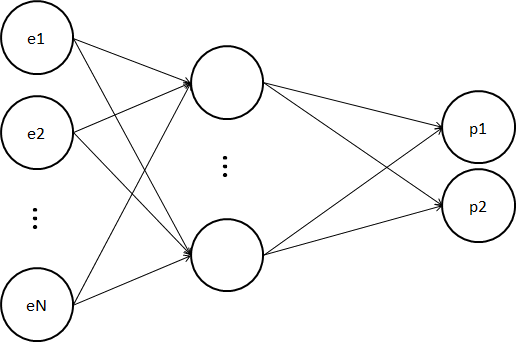
\includegraphics[scale=0.2]{imagenes/redNeuronal.png}
\label{fig:jug_redNeuronal}
\end{figure}
\end{column}
\end{columns}
}
\end{block}
\end{frame}

%%------------------------------------------------------------------------------
% Transparencia red neuronal
%\begin{frame}[squeeze]
%\frametitle{Red Neuronal}
%\begin{block}{}
%Red neuronal multicapa con aprendizaje mediante retropropagación.
%\begin{figure}[t]
%\centering
%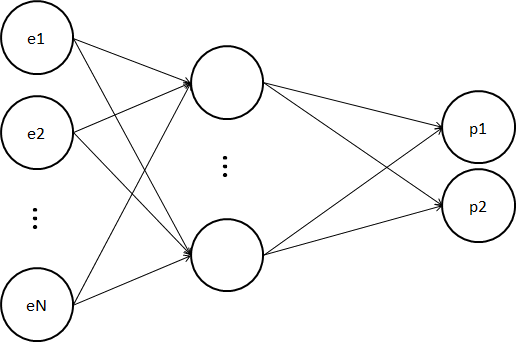
\includegraphics[scale=0.2]{imagenes/redNeuronal.png}
%\label{fig:jug_redNeuronal}
%\end{figure}
%\begin{displaymath}
%e(n) = p_1 - p_2
%\end{displaymath}
%Parámetros:
%\begin{itemize}
%\item Número neuronas intermedias
%\item Tasa de aprendizaje
%\item Momento
%\end{itemize}
%\end{block}
%\begin{alertblock}{}
%Depende de la codificación de los estados del juego.
%\end{alertblock}
%\end{frame}

%%------------------------------------------------------------------------------
% Transparencia heurísticos Conecta-K
\begin{frame}[t]
\frametitle{Heurísticos específicos de los juegos}

\begin{block}{Conecta-K}
\begin{itemize}
%\begin{columns}
%	\begin{column}{0.5\linewidth}
%	\begin{itemize}
%		\item Posibilidades 0, 1 y 2:
%		\begin{figure}[t]
%		\centering
%		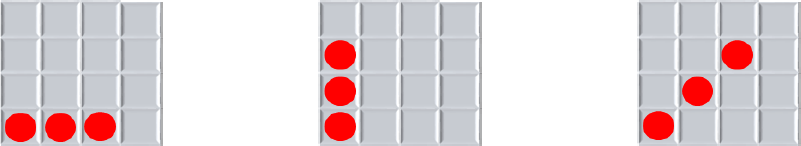
\includegraphics[scale=0.15]{imagenes/matrizPosibilidades1.png}
%		\label{fig:matrizPosibilidades1}
%		\end{figure}
%	\end{itemize}
%	\end{column}
%	\begin{column}{0.5\linewidth}
%		\begin{itemize}
%		\item Posibilidades 0, 1 y 2:
%		\begin{figure}[t]
%		\centering
%		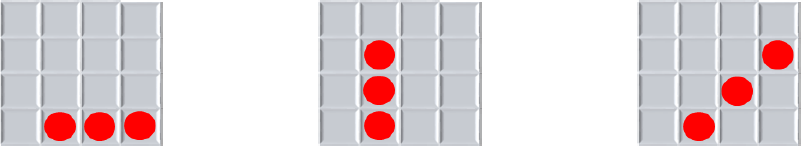
\includegraphics[scale=0.15]{imagenes/matrizPosibilidades2.png}
%		\label{fig:matrizPosibilidades2}
%		\end{figure}
%		\end{itemize}
%	\end{column}
%\end{columns}
%\begin{figure}[t]
%\centering
%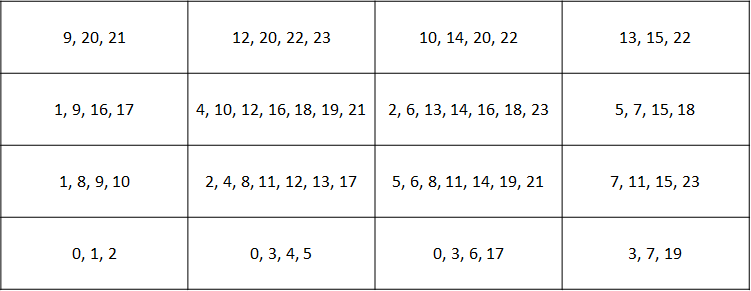
\includegraphics[scale=0.3]{imagenes/matrizPosibilidades.png}
%\label{fig:matrizPosibilidades}
%\end{figure}
\item \textbf{Matriz de posibilidades:}
\begin{center}
$e(n) = posibilidades_{MAX}(n)− posibilidades_{MIN}(n)$
\end{center}
\begin{center}
{\footnotesize
\begin{tabular}{|c|c|c|c|c|c|c|}
\hline
3& 4& 5& 7& 5& 4& 3\\ 
\hline
4& 6& 8& 10& 8& 6& 4\\ 
\hline
5& 8& 11& 13& 11& 8& 5\\ 
\hline
5& 8& 11& 13& 11& 8& 5\\ 
\hline
4& 6& 8& 10& 8& 6& 4 \\
\hline
3& 4& 5& 7& 5& 4& 3 \\
\hline
\end{tabular}
}
\end{center}

\end{itemize}
\end{block}

\begin{block}{Go}
\begin{itemize}
\item \textbf{Territorios:}
$e(n) = territorios_{MAX}(n) - territorios_{MIN}(n)$
\item \textbf{Puntos JP:}
$e(n) = puntos_{MAX}^{JP}(n) - puntos_{MIN}^{JP}(n)$
\item \textbf{Puntos CH:}
$e(n) = puntos_{MAX}^{CH}(n) - puntos_{MIN}^{CH}(n)$
\end{itemize}
\end{block}
\end{frame}

%%------------------------------------------------------------------------------
% Transparencia heurísticos Go
%\begin{frame}[t]
%\frametitle{Heurísticos para el Go}
%\begin{block}{Evaluador de territorios}
%\begin{displaymath}
%e(n) = territorios_{MAX}(n) - territorios_{MIN}(n)
%\end{displaymath}
%\end{block}
%
%\begin{block}{Evaluador de puntos JP}
%\begin{displaymath}
%e(n) = puntos_{MAX}^{JP}(n) - puntos_{MIN}^{JP}(n)
%\end{displaymath}
%\end{block}
%
%\begin{block}{Evaluador de puntos CH}
%\begin{displaymath}
%e(n) = puntos_{MAX}^{CH}(n) - puntos_{MIN}^{CH}(n)
%\end{displaymath}
%\end{block}
%
%\end{frame}

%%------------------------------------------------------------------------------
% La aplicación
\section{La aplicación}

% Transparencia aplicación
%\begin{frame}[t]
%\frametitle{El entorno interactivo}
%\begin{block}{Casos de uso}
%\begin{description}
%	\item[Jugar] 
%	\begin{itemize}
%	\item Contra otro jugador humano.
%	\item Contra cualquier estrategia.		
%	\item Ver el desarrollo de una partida entre dos agentes.
%	\end{itemize}
%	\item[Simular] un número determinado de partidas.
%	\item[Analizar] un estado concreto de un juego, estudiando el movimiento que realiza cada agente en ese estado.
%\end{description}
%
%En todos los casos se proporcionan estadísticas:
%\begin{itemize}
%\item Genéricas: propias del caso de uso.
%\item Específicas: de cada estrategia.
%\end{itemize}
%
%Posibilidad de generar un informe con las estadísticas.
%\end{block}
%
%\end{frame}

%%------------------------------------------------------------------------------
% CONCLUSIONES
\section{Conclusiones}

% Transparencia experimentos
\begin{frame}[t]
\frametitle{Evaluadores heurísticos en el Go}
{\large Jugador 1}
\begin{figure}[t]
\centering
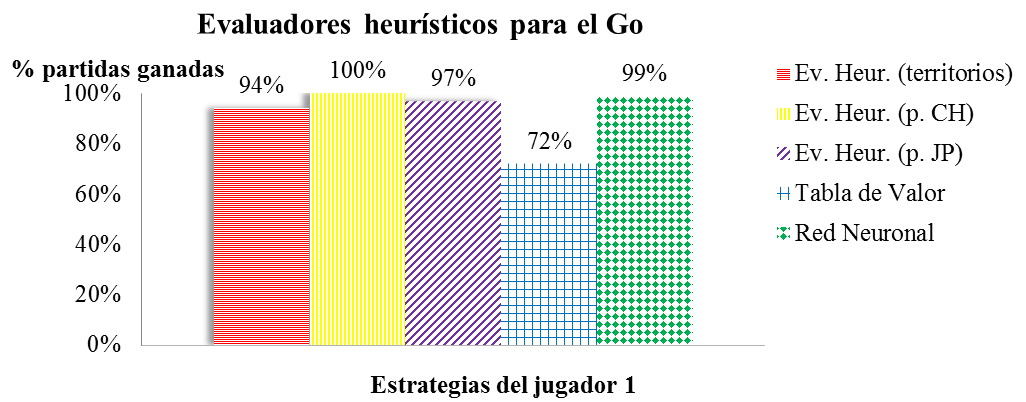
\includegraphics[scale=0.2]{imagenes/heuristicosGojug1.png}
\label{fig:heuristicosGojug1}
\end{figure}

{\large Jugador 2}
\begin{figure}[t]
\centering
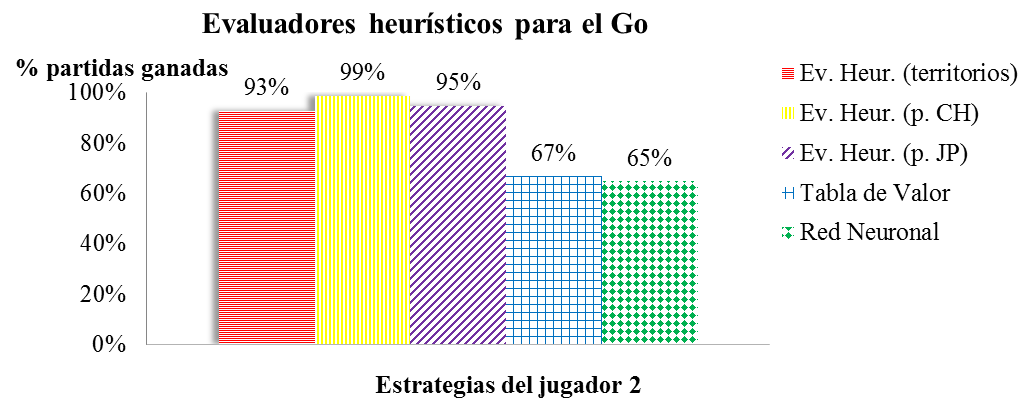
\includegraphics[scale=0.2]{imagenes/heuristicosGojug2.png}
\label{fig:heuristicosGojug2}
\end{figure}
\end{frame}

%%------------------------------------------------------------------------------
% Transparencia experimentos
\begin{frame}[t]
\frametitle{Estrategias en el Go}
{\large Jugador 1}
\begin{figure}[t]
\centering
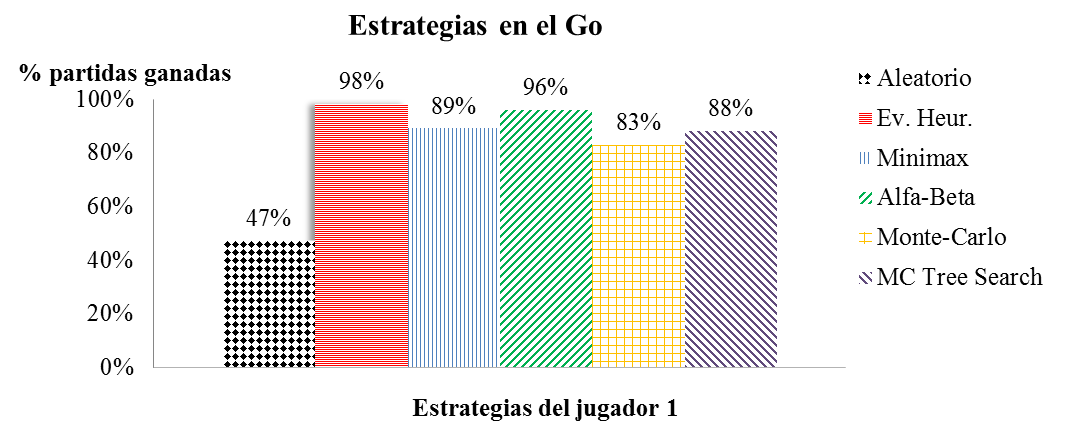
\includegraphics[scale=0.2]{imagenes/estrategiasGo1.png}
\label{fig:estrategiasGo1}
\end{figure}

{\large Jugador 2}
\begin{figure}[t]
\centering
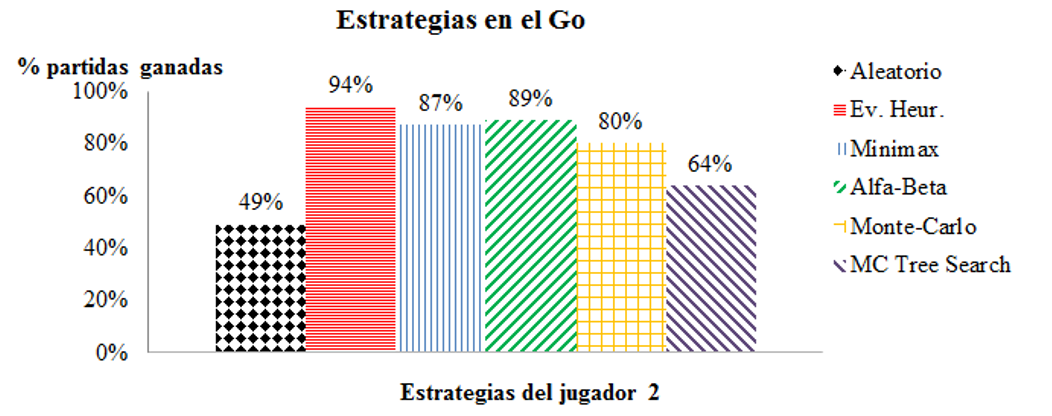
\includegraphics[scale=0.2]{imagenes/estrategiasGo2.png}
\label{fig:estrategiasGo2}
\end{figure}
\end{frame}

% Transparencia conclusiones
\begin{frame}[t]
\frametitle{Conclusiones y trabajo futuro}
\begin{block}{Conclusiones}
%\begin{itemize}
%	\item La búsqueda de una estrategia óptima es un problema intratable.
%	\item Los algoritmos deben hacer algunas suposiciones y aproximaciones.
%\end{itemize}

\begin{itemize}
	\item Herramienta didáctica para estudiar, analizar y comparar algoritmos.
	\item Marco de trabajo.
\end{itemize}
\end{block}

\begin{block}{Trabajo futuro}
\begin{columns}
\begin{column}{0.5\linewidth}
\begin{itemize}
	\item Adaptación del módulo de razonamiento a otras clases de juegos.
	\item Nuevos algoritmos.
	%\item Mejoras en la aplicación.
\end{itemize}
\end{column}
\begin{column}{0.5\linewidth}
\begin{figure}[t]
\centering
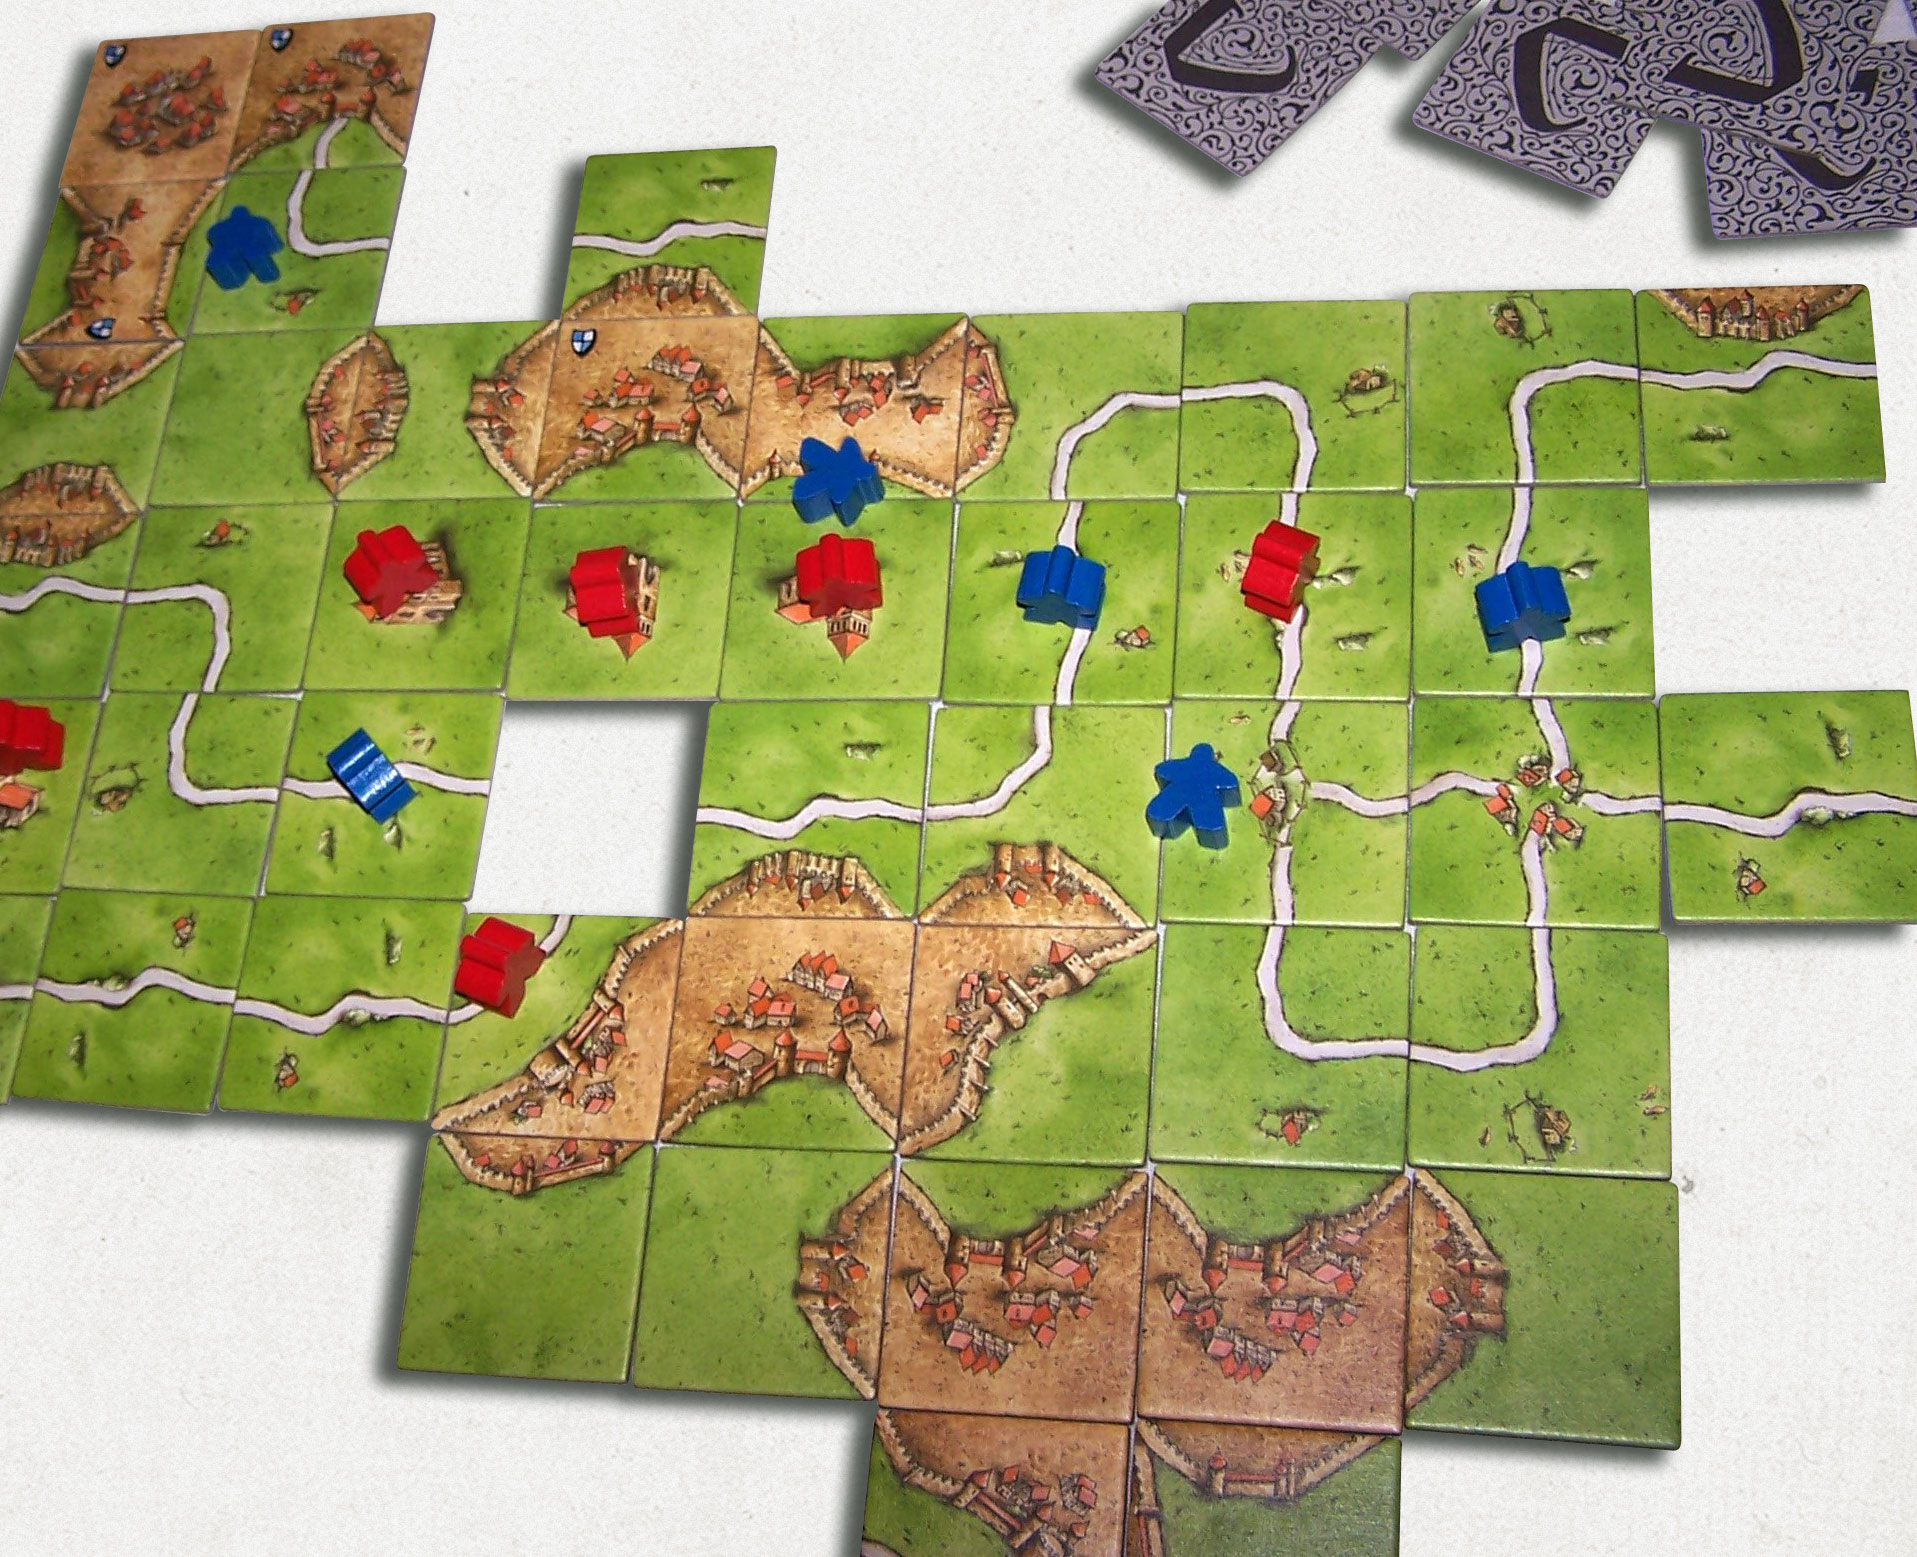
\includegraphics[scale=0.05]{imagenes/carcassonne.png}
\label{fig:carcassonne}
\end{figure}
\end{column}
\end{columns}
\end{block}

\end{frame}


\end{document}		% fin documento
